\documentclass[11pt]{article}
\usepackage[utf8]{inputenc}
\usepackage{graphicx}
\usepackage[space,extendedchars]{grffile}
\usepackage{float}
\usepackage{hyperref}
\usepackage{geometry}
\usepackage{booktabs}
\usepackage{subcaption}
\usepackage{xcolor}
\usepackage{fancyhdr}
\usepackage{titlesec}
\usepackage{enumitem}
\usepackage{amsmath}
\usepackage{microtype}

% Slightly relax line breaking
\emergencystretch=2em

\geometry{margin=1in, top=1.2in, bottom=1.2in}

% Image search paths (handles directories with spaces)
\graphicspath{{./figures/}{../JupyterOutputs/}{../JupyterOutputs/Clustering (SpatialHotspots)/}{../JupyterOutputs/Classification (Final)/}{../JupyterOutputs/PatternAnalysis/}{../Application/Police/}}

% Header and footer
\pagestyle{fancy}
\fancyhf{}
\fancyhead[L]{Crime Analyzer}
\fancyhead[R]{Police Dashboard Guide}
\fancyfoot[C]{\thepage}
\setlength{\headheight}{14pt}

% Section formatting
\titleformat{\section}{\Large\bfseries\color{black}}{\thesection}{1em}{}
\titleformat{\subsection}{\large\bfseries}{\thesubsection}{1em}{}

% Hyperlink setup
\hypersetup{
    colorlinks=true,
    linkcolor=black,
    urlcolor=black,
    citecolor=green!50!black
}

\title{\Huge\textbf{Police Intelligence Dashboard}\\[2mm]
       \Large\textit{User Guide for Operational Use}}
\author{\textit{Crime Analyzer Platform}}
\date{\today}

\begin{document}

\maketitle
\tableofcontents
\newpage

% ===================== 1. Executive Summary =====================
\section{Executive Summary}

\subsection{System Overview}
The Police Intelligence Dashboard is an operations-facing interface designed to quickly surface crime hotspots, priority patterns, and clear recommendations. It integrates a map-based hotspot view with key performance indicators (KPIs) and pattern insights produced by clustering and association-rule analysis.

\subsection{Key Capabilities}
\begin{itemize}[leftmargin=*]
  \item Hotspot visualization of spatio-temporal clusters.
  \item Executive KPIs summarizing clustering outputs.
  \item Priority patterns with plain-language summaries.
  \item Actionable recommendations for deployment and prevention.
  \item Pattern Analysis modal with global, borough, and time-bucket insights.
\end{itemize}

\subsection{Target Users}
\begin{itemize}[leftmargin=*]
  \item \textbf{Police operations and analysts:} For situational awareness and resource allocation.
  \item \textbf{Command staff:} For strategy and deployment decisions based on patterns and trends.
\end{itemize}

% ===================== 2. Quick Start Guide =====================
\section{Quick Start Guide}

\subsection{Accessing the Dashboard}
Open the Police Intelligence Dashboard by launching \texttt{Application/Police/index.html}. Ensure the images under \texttt{Documents/figures/} and \texttt{JupyterOutputs/} are present so all panels render correctly.

\subsection{Daily Workflow in 3 Steps}
\begin{enumerate}
  \item \textbf{Scan hotspots:} Start from the map to see where activity concentrates and when.
  \item \textbf{Read KPIs and patterns:} Use the cards and priority patterns to gauge intensity and focus areas.
  \item \textbf{Zoom with Pattern Analysis:} Open the modal, choose a borough and time bucket, and review the top rules in plain language.
\end{enumerate}

\subsection{How to Interpret}
\begin{itemize}[leftmargin=*]
  \item \textbf{Hotspot Map:} Highlights locations and time windows with the highest concentration. Use it to position patrols and define coverage.
  \item \textbf{KPIs:} Total volume, patterns identified, number and share of high-priority patterns. These provide an at-a-glance workload indicator.
  \item \textbf{Priority Patterns:} Two spotlights: \emph{Most concentrated} (tightest cluster) and \emph{Highest volume} (largest case count). Each includes crime type, borough, premises, time bucket, and, when available, suspect/victim modes.
  \item \textbf{Recommendations:} Action cues derived from the executive summary (e.g., deploy in specific premises or borough; schedule afternoon rotations).
  \item \textbf{Pattern Analysis Modal:} Global, Borough, and Time views list the strongest rules with strength badges (confidence, lift, support) and a short outcome sentence.
\end{itemize}

% ===================== 3. How the Dashboard Works =====================
\section{Dashboard Panels and Navigation}

\subsection{Hotspot Map}
A map view of spatial clusters with temporal patterns. Use it to:
\begin{itemize}[leftmargin=*]
  \item Identify persistent hotspots.
  \item Note peak windows (morning, afternoon, evening, night).
  \item Cross-check with known events or seasonal effects.
\end{itemize}

\begin{figure}[H]
  \centering
  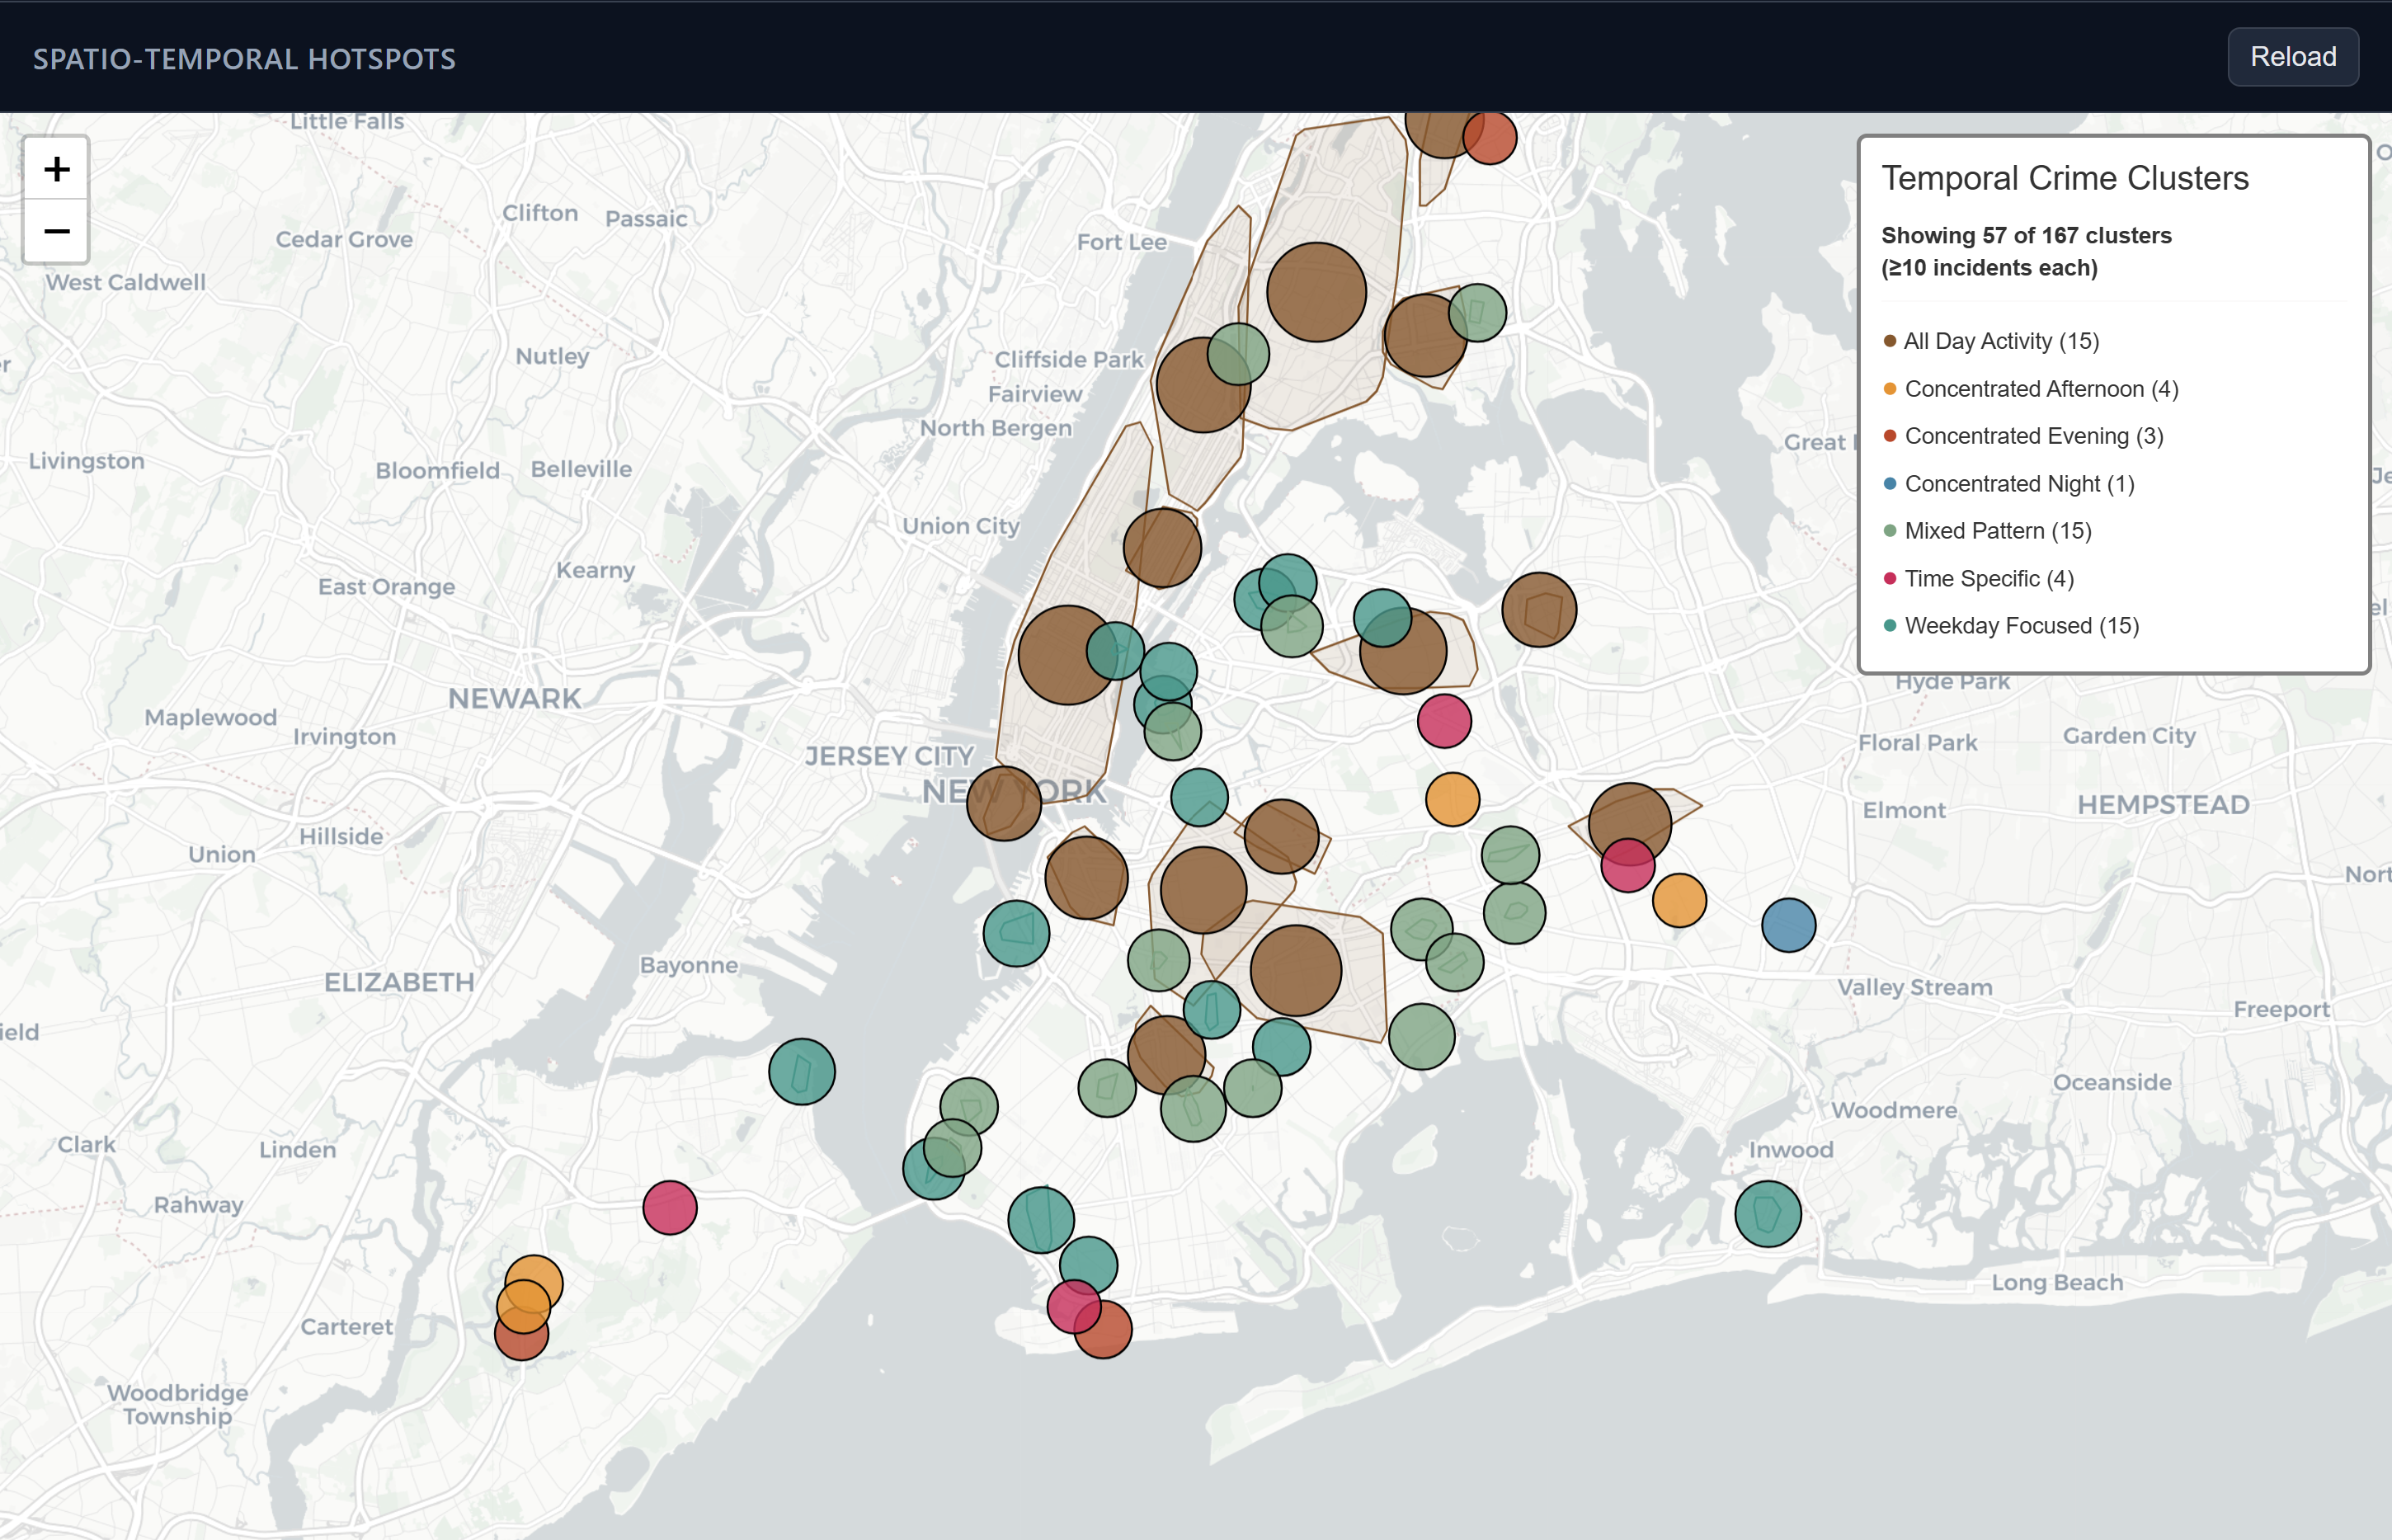
\includegraphics[width=0.98\textwidth]{spatio-temporal_clusters.png}
  \caption{Example of spatio-temporal hotspots as visualized in the dashboard map.}
\end{figure}

\subsection{Executive KPIs}
Cards summarize \emph{Crimes analyzed}, \emph{Patterns identified}, \emph{High-priority patterns}, and \emph{\% High-priority crimes}. Rising counts suggest wider or denser clusters. A higher share of high-priority patterns signals where to focus near-term action.

\subsection{Priority Patterns}
Two pattern spotlights:
\begin{itemize}[leftmargin=*]
  \item \textbf{Most concentrated:} Highest density within a narrow area/time.
  \item \textbf{Highest volume:} Largest number of cases.
\end{itemize}
Each pattern shows crime type, borough, premises, time bucket, weekday/weekend mode, and typical suspect/victim attributes when informative.

\subsection{Recommendations}
Automatic cues that translate insights into actions. Examples: deploy targeted patrols over the next 7 days in afternoon windows; coordinate precincts in a specific borough; engage premises owners for prevention.

\subsection{Pattern Analysis Modal}
Explore the strongest association rules:
\begin{itemize}[leftmargin=*]
  \item \textbf{Views:} Global, Borough, Time.
  \item \textbf{Filters:} Borough chips (Manhattan, Brooklyn, Bronx, Queens, Staten Island) and time chips (Morning, Afternoon, Evening, Night).
  \item \textbf{Rule strength:} Each rule shows confidence (\%), lift, and support; weaker rules are filtered out.
\end{itemize}

\subsubsection*{Interpreting Pattern Rules}
Rules are presented as \texttt{IF (conditions) THEN (outcome)} and summarize when a given outcome becomes more likely. Read them as guidance about \emph{context}, not causation.
\begin{itemize}[leftmargin=*]
  \item \textbf{Premises (IF):} Conditions such as borough, time bucket, premises type, and contextual factors that define a situation of interest.
  \item \textbf{Outcome (THEN):} The category that becomes more likely under those conditions.
  \item \textbf{Confidence (\%):} Among incidents matching the premises, the percentage where the outcome also occurs (e.g., 72\% means roughly 72 in 100).
  \item \textbf{Lift:} How much more likely the outcome is compared with its baseline occurrence citywide (e.g., 1.30 \(\Rightarrow\) 30\% more likely).
  \item \textbf{Support:} Prevalence of the rule in the dataset (share of all incidents matching both premises and outcome).
  \item \textbf{Ranking metrics:} Kulc/Score help order rules; prioritize high confidence and lift with reasonable support.
\end{itemize}

\noindent\textit{Example.}\; \texttt{IF (BORO = MANHATTAN) AND (TIME\_BUCKET = EVENING) THEN (PREMISES = RESTAURANT)}\\
\quad Metrics: Conf 72\%, Lift 1.30, Support 0.18.\\
\emph{Interpretation:} In Manhattan evenings, restaurant-related incidents occur more often than baseline (about 30\% higher) and cover a meaningful share of incidents. Combine with the hotspot map and KPIs to plan patrol timing and engagement with premises.

% ===================== 4. How the system works =====================
\section{How the System Works}

\subsection{Spatio-Temporal Clustering}
Incidents are grouped by geographic proximity and time-of-day windows. The method highlights compact areas that show recurring concentration. Outputs include hotspot centroids, indicative area spreads, and peak time buckets (morning, afternoon, evening, night). These inform patrol placement and scheduling decisions.

\subsection{Multidimensional Clustering}
Beyond location and time, the analysis considers additional attributes (e.g., premises type and contextual factors) to surface cohesive patterns. The executive layer synthesizes these clusters into KPIs (total volume, identified patterns, high-priority share) and spotlights representative patterns most relevant to operations.

\subsection{Pattern Analysis}
Association rules summarize condition $\rightarrow$ outcome relationships in simple sentences (e.g., \emph{"Retail-related incidents are more likely when conditions X and Y co-occur"}). Each rule is shown with confidence, lift, and support. We filter to favor stronger evidence.

% ===================== 5. Data and Analysis =====================
\section{Data and Analysis}

\subsection{Data Overview}
Analyses use historical complaint data enriched with temporal (hour, weekday/weekend, time bucket) and contextual features. These enable discovery of patterns across space, time, and operational contexts.

\subsection{Data Sources}
The analyses are grounded in reliable, comprehensive sources:
\begin{itemize}[leftmargin=*]
  \item \textbf{NYPD Complaint Data:} Historical and current crime reports from the New York City Police Department.
  \item \textbf{Geographic Data:} Points of Interest (POI), such as transit stations, commercial establishments, and schools.
\end{itemize}

\subsection{Data Processing}
To ensure accuracy, the raw data undergo rigorous preparation: cleaning, handling missing values, and integrating information from multiple sources. This is crucial for stable clustering and reliable pattern discovery.

\subsection{Preprocessing and Feature Engineering}
\begin{itemize}[leftmargin=*]
  \item Standardization of time features (hour bands, weekday/weekend).
  \item Geographic normalization for clustering stability.
  \item Categorical encoding for premises and other contextual fields.
\end{itemize}

\subsection{Analysis Outputs}
\begin{itemize}[leftmargin=*]
  \item Hotspot clusters with peak windows.
  \item KPI summary with high-priority share.
  \item Priority patterns (most concentrated, highest volume).
  \item Top association rules by global, borough, and time bucket views.
\end{itemize}

% ===================== 6. Model validation =====================
\section{Model Validation}

\subsection{Cluster Quality}
Configurations are assessed with complementary diagnostics and practical criteria. We use the \textbf{silhouette score} to gauge cohesion and separation: incidents should be closer to their own cluster than to others. The \textbf{k-distance (k-dist) plot} provides an elbow that guides density or neighborhood parameters; thresholds are set near clear inflection points. Beyond numeric indices, we prioritize \emph{operational interpretability}: clusters should be spatially compact and contiguous, align with recognizable geography (e.g., transit hubs, retail corridors), and exhibit \textbf{temporal coherence} (clear peak windows rather than diffuse activity across all times). Finally, we check \textbf{stability} by verifying that salient hotspots persist across resampled subsets and adjacent time slices.

For \textbf{multidimensional clustering}, evaluation focuses on internal separation/cohesion (e.g., silhouette), \emph{parsimony} in the number of segments, and \textbf{interpretability} of the resulting profiles (consistent combinations of crime type, premises, borough, and time bucket). We prefer compact, well-separated segments that cover a meaningful share of incidents and remain stable under light resampling.

\begin{figure}[H]
  \centering
  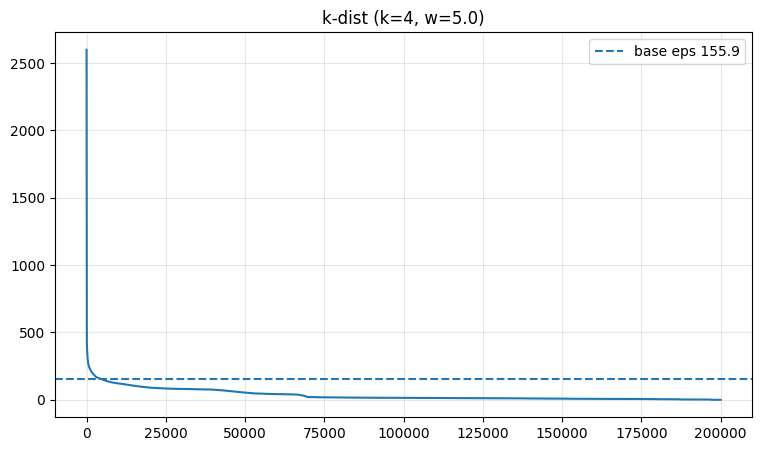
\includegraphics[width=0.9\textwidth]{k-dist.png}
  \caption{k-dist (k-distance) plot used to select density/neighborhood parameters for clustering.}
\end{figure}

\subsection{Rule Strength}
Displayed rules are screened by thresholds (confidence, lift, support) to prioritize reliable associations and reduce noise.

% ===================== 7. Responsible Use and Ethics =====================
\section{Responsible Use and Ethics}

\subsection{Ethical Principles}
\begin{itemize}[leftmargin=*]
  \item \textbf{Non-individualization:} Use insights to guide locations, times, and premises for prevention; do not infer individual culpability.
  \item \textbf{Fairness:} Demographic attributes are descriptive of historical data and must not be used for targeting or discriminatory enforcement.
  \item \textbf{Transparency:} Communicate that associations indicate context, not causation; present rule strengths (confidence, lift, support).
  \item \textbf{Community engagement:} Incorporate local knowledge and community input when interpreting patterns.
\end{itemize}

\subsection{Operational Guidance}
\begin{itemize}[leftmargin=*]
  \item Combine dashboard insights with officer expertise and recent incident reports before acting.
  \item Review outputs periodically to detect drift or unintended effects; update tactics accordingly.
  \item Document key deployment decisions and their rationale when driven by pattern insights.
\end{itemize}

% ===================== 8. System Limitations =====================
\section{System Limitations}

\subsection{Known Constraints}
\begin{itemize}[leftmargin=*]
  \item \textbf{Historical basis:} Patterns reflect past data and may shift with events, policy changes, or seasonality.
  \item \textbf{Data quality:} Missing or noisy attributes can affect clustering and rules.
  \item \textbf{Granularity:} Time buckets and spatial resolution trade off detail and stability.
  \item \textbf{Interpretation:} Associations are correlational; use with operational judgment.
\end{itemize}

\subsection{Risk Mitigation}
\begin{itemize}[leftmargin=*]
  \item Cross-check with recent incident logs and officer observations before acting.
  \item Note unusual events (holidays, disruptions) that may temporarily shift conditions.
  \item Prefer tactics that are reversible and review outcomes regularly to refine deployment.
\end{itemize}

% ===================== 9. FAQ =====================
\section{FAQ}

\subsection*{How often should we revisit the dashboard?}
Daily for hotspot scanning; weekly for reviewing pattern rules and adjusting tactics.

\subsection*{What indicates immediate action?}
A surge in high-priority share, a new dense hotspot, or consistent strong rules around a premises/time.

\subsection*{Can we compare boroughs quickly?}
Yes. Use the Pattern Analysis modal's borough view and read the strongest rules per borough.

\subsection*{How do we choose shift times?}
Align patrol windows with hotspot peak time buckets and the recommendations panel.

\subsection*{Do rules target individuals?}
No. Rules describe context patterns; they must not be used for individual targeting.

% ===================== 10. Future Enhancements =====================
\section{Future Enhancements}
\begin{itemize}[leftmargin=*]
  \item Near-real-time refresh and alerting when thresholds are exceeded.
  \item Seasonal and event-aware models to adapt to city calendars.
  \item Comparative views across weeks and precincts with trend lines.
  \item What-if tools to test deployment changes against recent patterns.
\end{itemize}

% ===================== 11. Conclusion =====================
\section{Conclusion}
The Police Intelligence Dashboard unifies hotspots, executive indicators, and explainable patterns into a single operational view. Used alongside officer expertise and community knowledge, it supports timely, targeted prevention and efficient allocation of resources.
\end{document}